% !TeX root = ../thesis.tex

\chapter{System}
\label{sec:system}

\section{Analoge Signalverarbeitung}
\label{sec:Signalverarbeitung}
Bei der Signalübertragung über den optischen Kanal mit dem in dieser Arbeit gewählten Medium Licht, müssen einige grundlegende Dinge beachtet werden. Im Kapitel~\ref{sub:led} der Leuchtdiode wurden ihre grundlegenden Eigenschaften erklärt, die es sich hier nun zu verwenden gilt. Eine bekannte Schwierigkeit ist die Übertragung von negativen Wellen. Diese können nicht Übertragen werden, da Licht keinen negativen Wert annehmen kann. Hinzu ist man bei der Übertragung von Signalen darauf bedacht, nur im linearen Bereich der LED-Kennlinie Daten zu übertragen. Wenn man diese nämlich im nichtlinearen Bereich der LED Überträgt, können Verzerrungen auftreten und somit die Übertragung stark gestört werden. Um jenes Problem zu lösen, wird ein Offset verwendet, welcher das Signal so positiv verschiebt, dass dieses keine negativen Anteile mehr besitzt. Zudem wurde ein Spannungspuffer eingerichtet um zusätzlich die Amplitude zu verstärken. Dies liefert Gewissheit, dass nur positive Spannungsanteile übertragen werden und somit kein Signalverlust verzeichnet werden muss.

\begin{figure}[H]
	\centering
	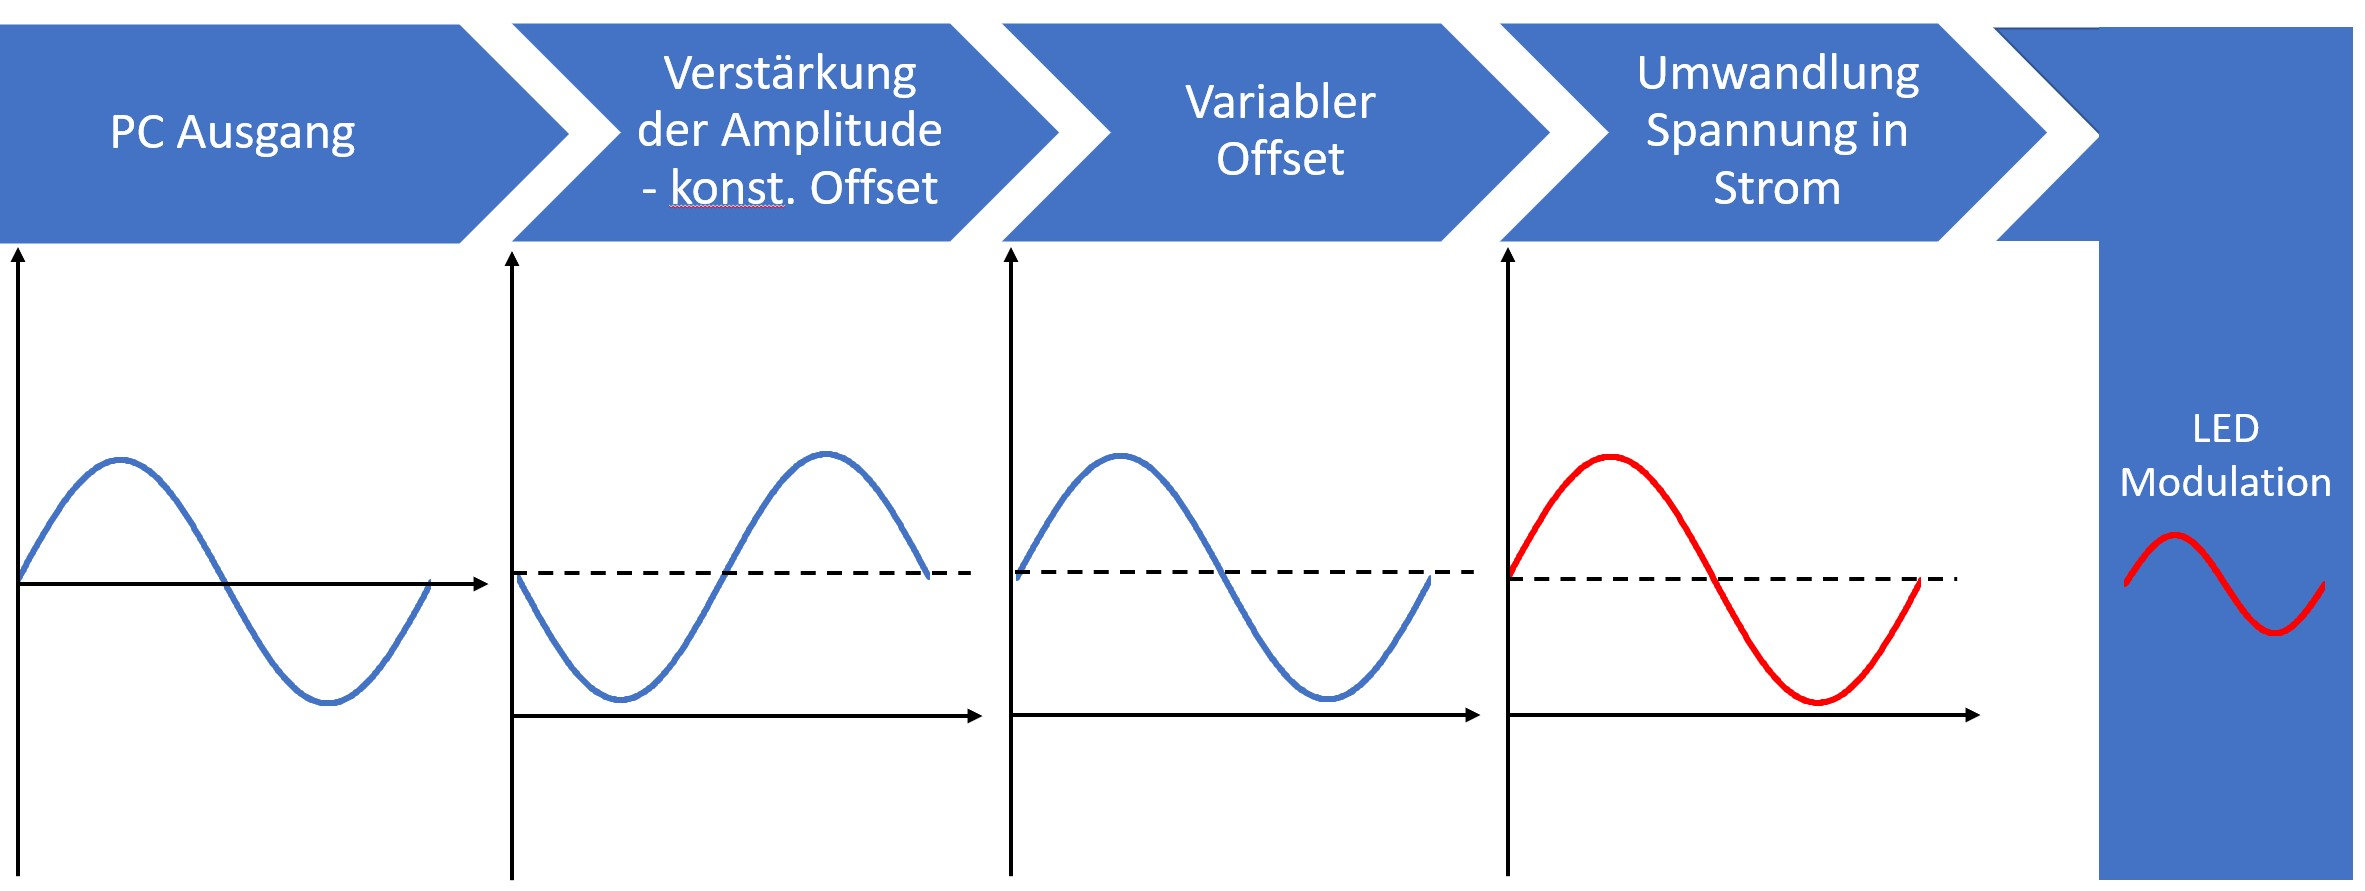
\includegraphics[width = 0.9 \textwidth ]{signalvorgang.jpg}
	\caption[Signalverarbeitungsschritte]{Signalverarbeitungsschritte} \gls{online:Eigen}
	\label{fig:signalvorgang}
\end{figure}

In Abbildung ~\ref{fig:signalvorgang} werden die Verschiedenen Stufen der Signalübertragung veranschaulicht. Da es sich an dieser Stelle um ein nichtlineares System handelt, dürfen die Signalverarbeitungsstufen nicht beliebig vertauscht werden. Eine solche Veränderung der Reihenfolge könnte zur Verfälschung des Signals führen. 

Die analoge Signalverarbeitungsschaltung wurde in drei Stufen aufgeteilt. Die \gls{acr:OP}- Grundschaltungen wurden hierfür so modifiziert, dass Amplitude und Offset variabel einstellbar sind und möglich auftretende Fehler vermieden werden. In Abbildung ~\ref{fig:stufe1} ist die Eingangssignalverarbeitungsstufe illustriert. 

\begin{figure}[H]
	\centering
	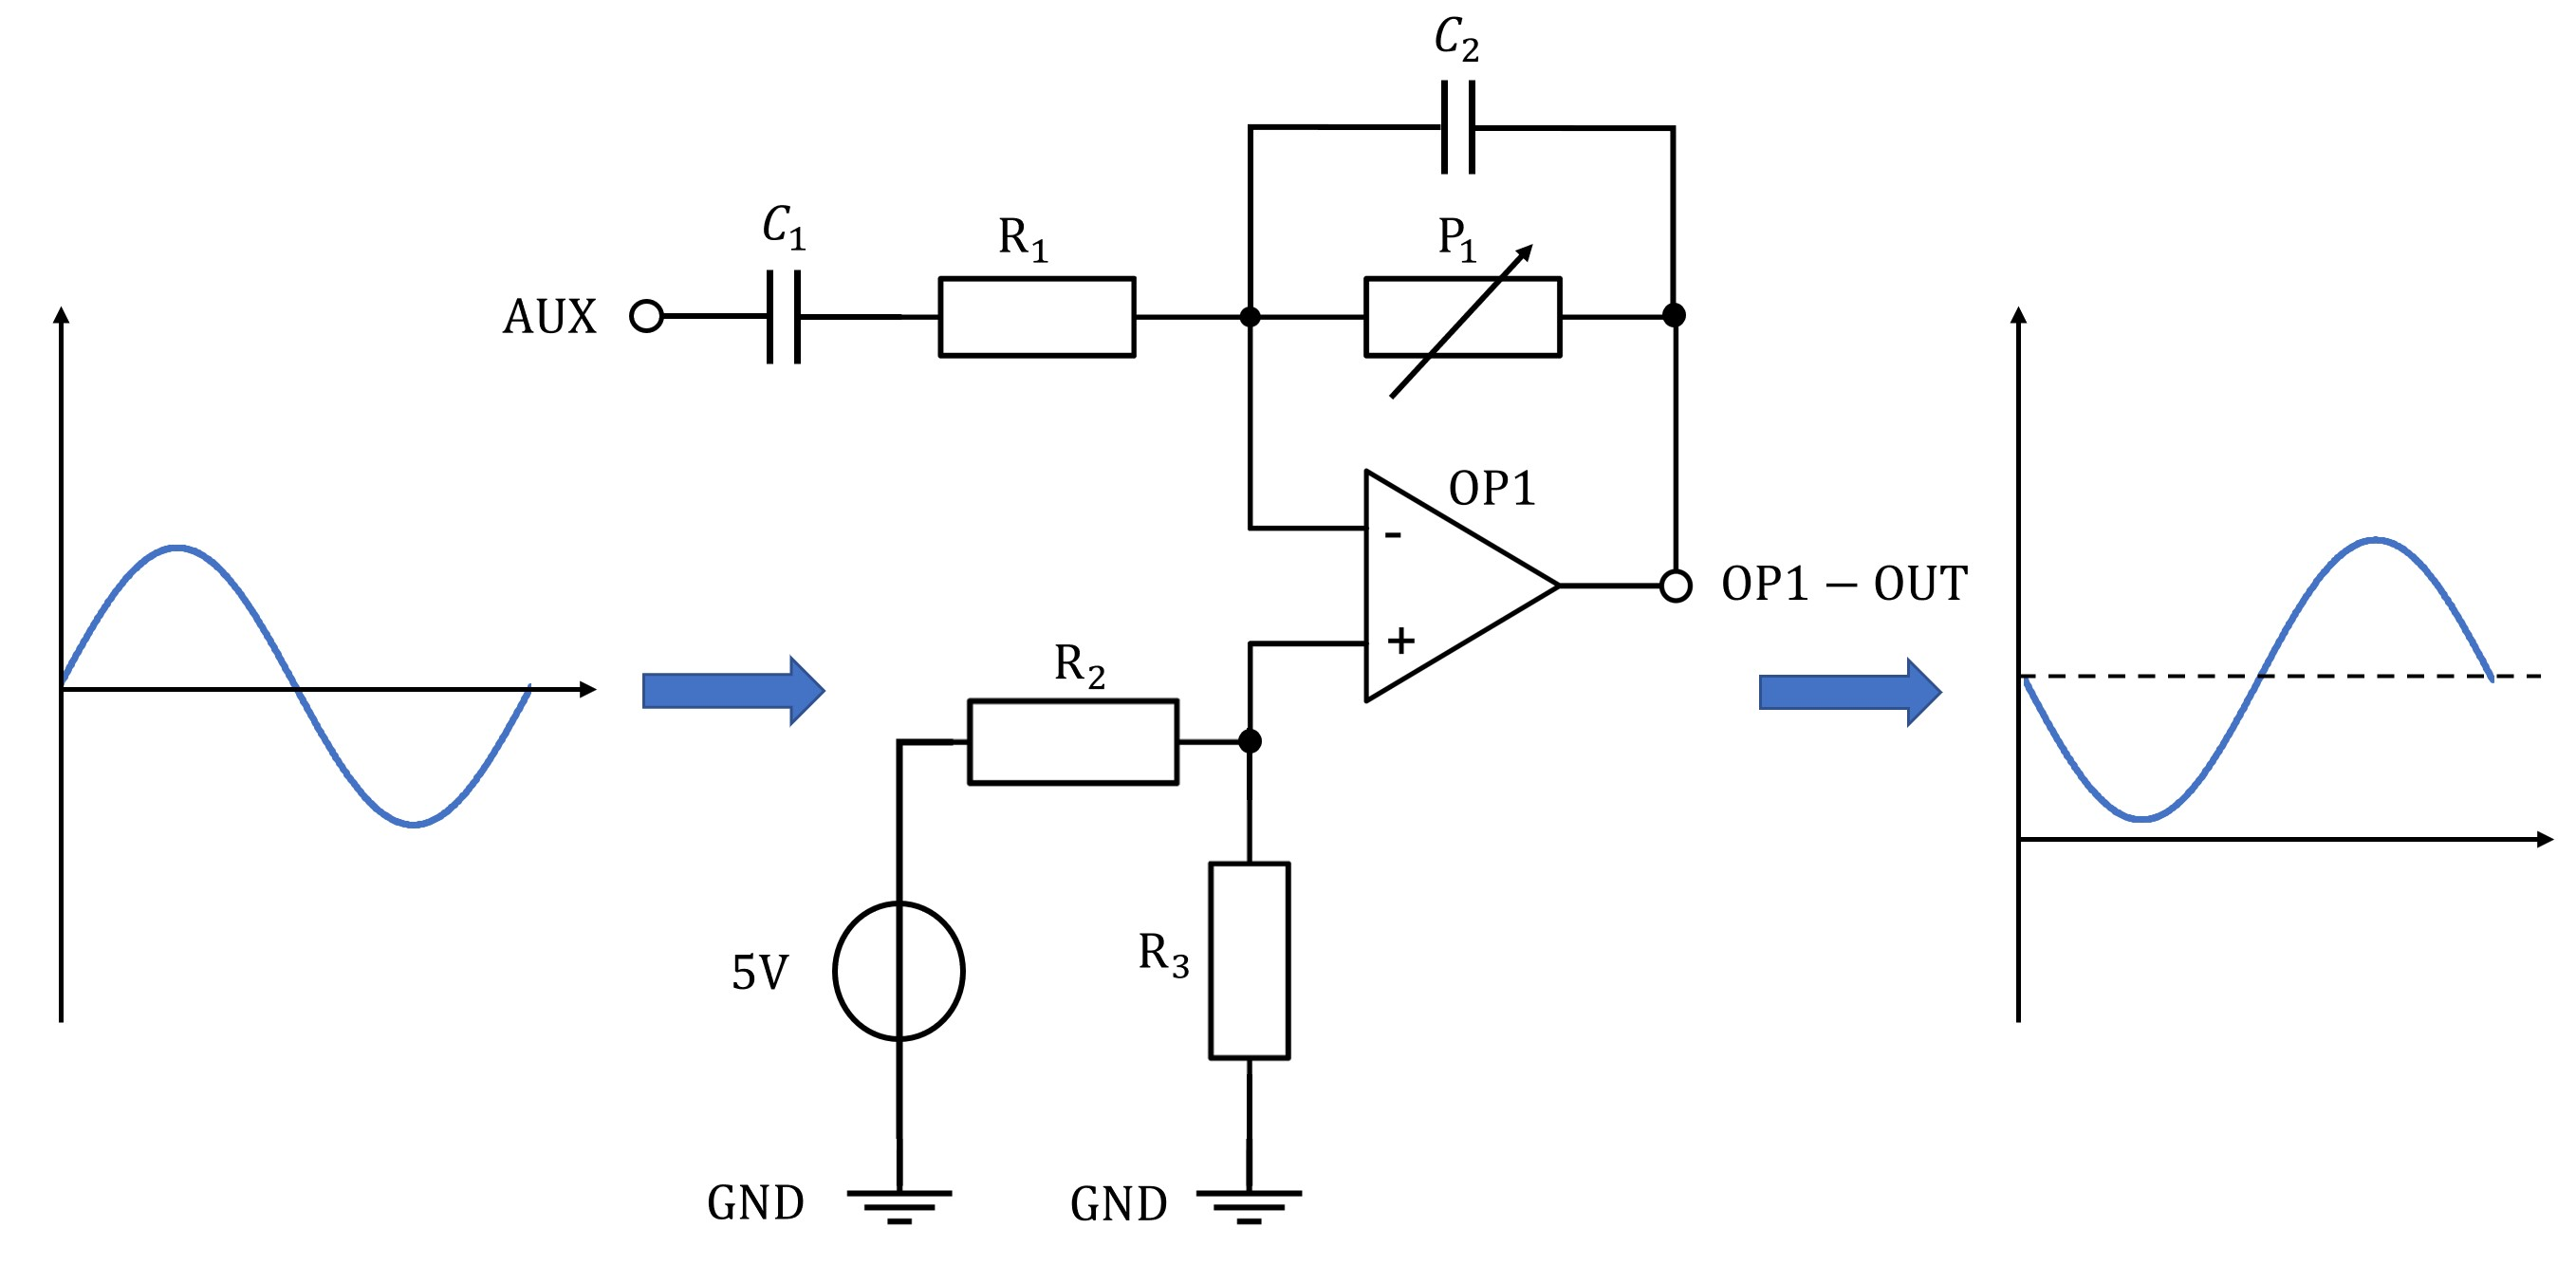
\includegraphics[width = 0.9 \textwidth ]{stufe1.jpg}
	\caption[Eingangssignalverarbeitungsstufe]{Eingangssignalverarbeitungsstufe} \gls{online:Eigen}
	\label{fig:stufe1}
\end{figure}

Der Schlüsselfaktor in der Eingangsstufe ist der variable Widerstand im Rückkopplungspfad des \gls{acr:OP}s. Hierbei handelt es sich um ein Digitales Potentiometer, welches sich über \gls{acr:SPI} vom Arduino zur Laufzeit beliebig verändern lässt. Die Schwierigkeit in der Implementierung dieses Bauteiles liegt jedoch darin, dass es keine negativen Spannungen verträgt. Aus dem Datenblatt ist ersichtlich, dass es nur mit Spannungen von $-0,6V<U<6V$ sorgfältig arbeiten kann. Da es sich bei dem zu verarbeitenden Audiosignal um ein Wechselstromsignal mit einer Amplitude von etwa 1,5V handelt, wurden in dieser Schaltung Vorkehrungen getroffen um die negativen Anteile dieses Signals in positive Anteile zu konvertieren. Um dieses Vorhaben zu realisieren wurde auf den nichtinvertierenden Eingang des \gls{acr:OP}s mithilfe eines Spannungsteilers $R_{3}$ und $R_{2}$ eine Spannung angelegt. Diese soll das Potential des \gls{acr:OP}s so anheben, dass das AC-Signal aus der Soundkarte direkt mit einem Offset addiert wird und somit keine negativen Anteile mehr besitzt. Um die Soundkarte vor der DC-Spannung zu schützen wurde ein DC Abblockkondensator $C_{1}$ am Signaleingang vorgesehen. Dieser ist für AC-Signale komplett durchlässig. Aufgrund der Annahme einer maximalen Amplitude von 1,5V muss also also ein Mindestoffset von 0,9V auf das Signal addiert werden. Um hier jedoch die Amplitude trotz Verstärkung innerhalb des erlaubten Spannungsbereiches von $-0,6V<U<6V$ bleiben wurde ein fester Offset von 2,15V gewählt. Zudem würde eine maximale Verstärkung von $A=2$ hinzugezogen wodurch sich der Spannungsbereich, selbst bei einer maximalen Verstärkung, stets in einem Bereich von $-0,2V<U<5,7V$ befindet. Dies ist in ~\ref{fig:ampoff} illustriert. 


\begin{figure}[H]
	\centering
	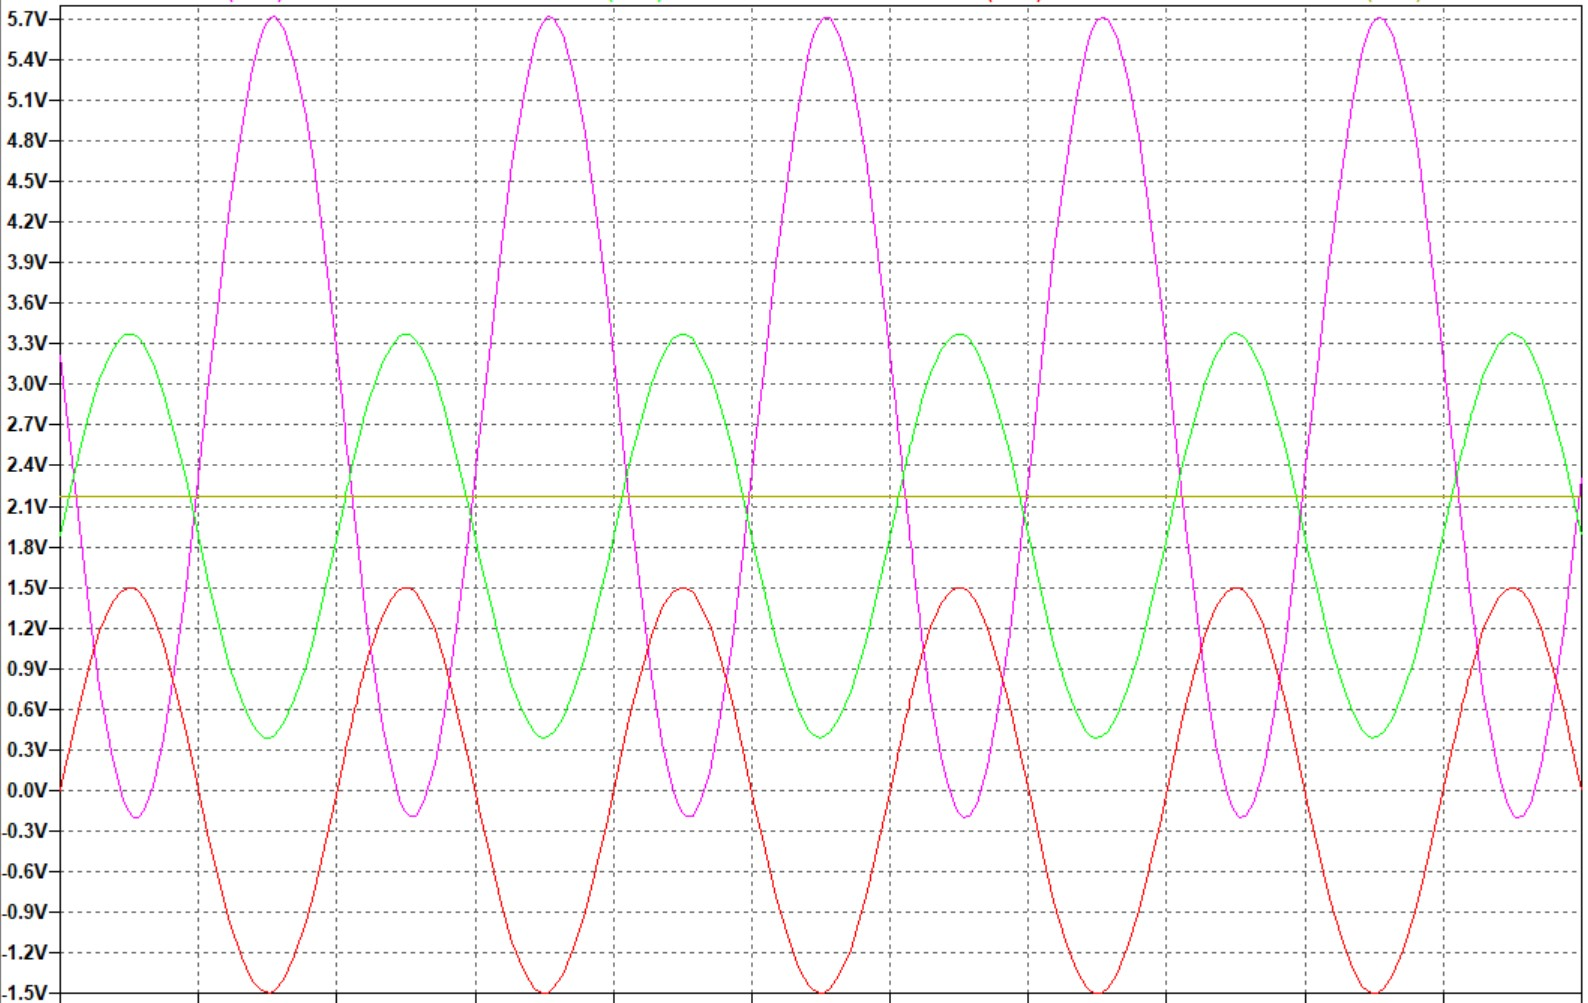
\includegraphics[width = 0.9 \textwidth ]{ampoff.jpg}
	\caption[Simulation von Offset und Verstärkung]{Simulation von Offset und Verstärkung} \gls{online:Eigen}
	\label{fig:ampoff}
\end{figure}

Somit kann gewährleistet werden, dass das Digitale Potentiometer zunehmend in einem legitimen Spannungsbereich betrieben wird.

Der zweite \gls{acr:OP} der Schaltung sorgt in der Signalkette für einen weiteren
Offset welcher die Grundhelligkeit der \gls{acr:LED} regelt. Da hier keine negative Spannung auftritt, kann das Digitale Potentiometer direkt angeschlossen werden.
\begin{figure}[H]
	\centering
	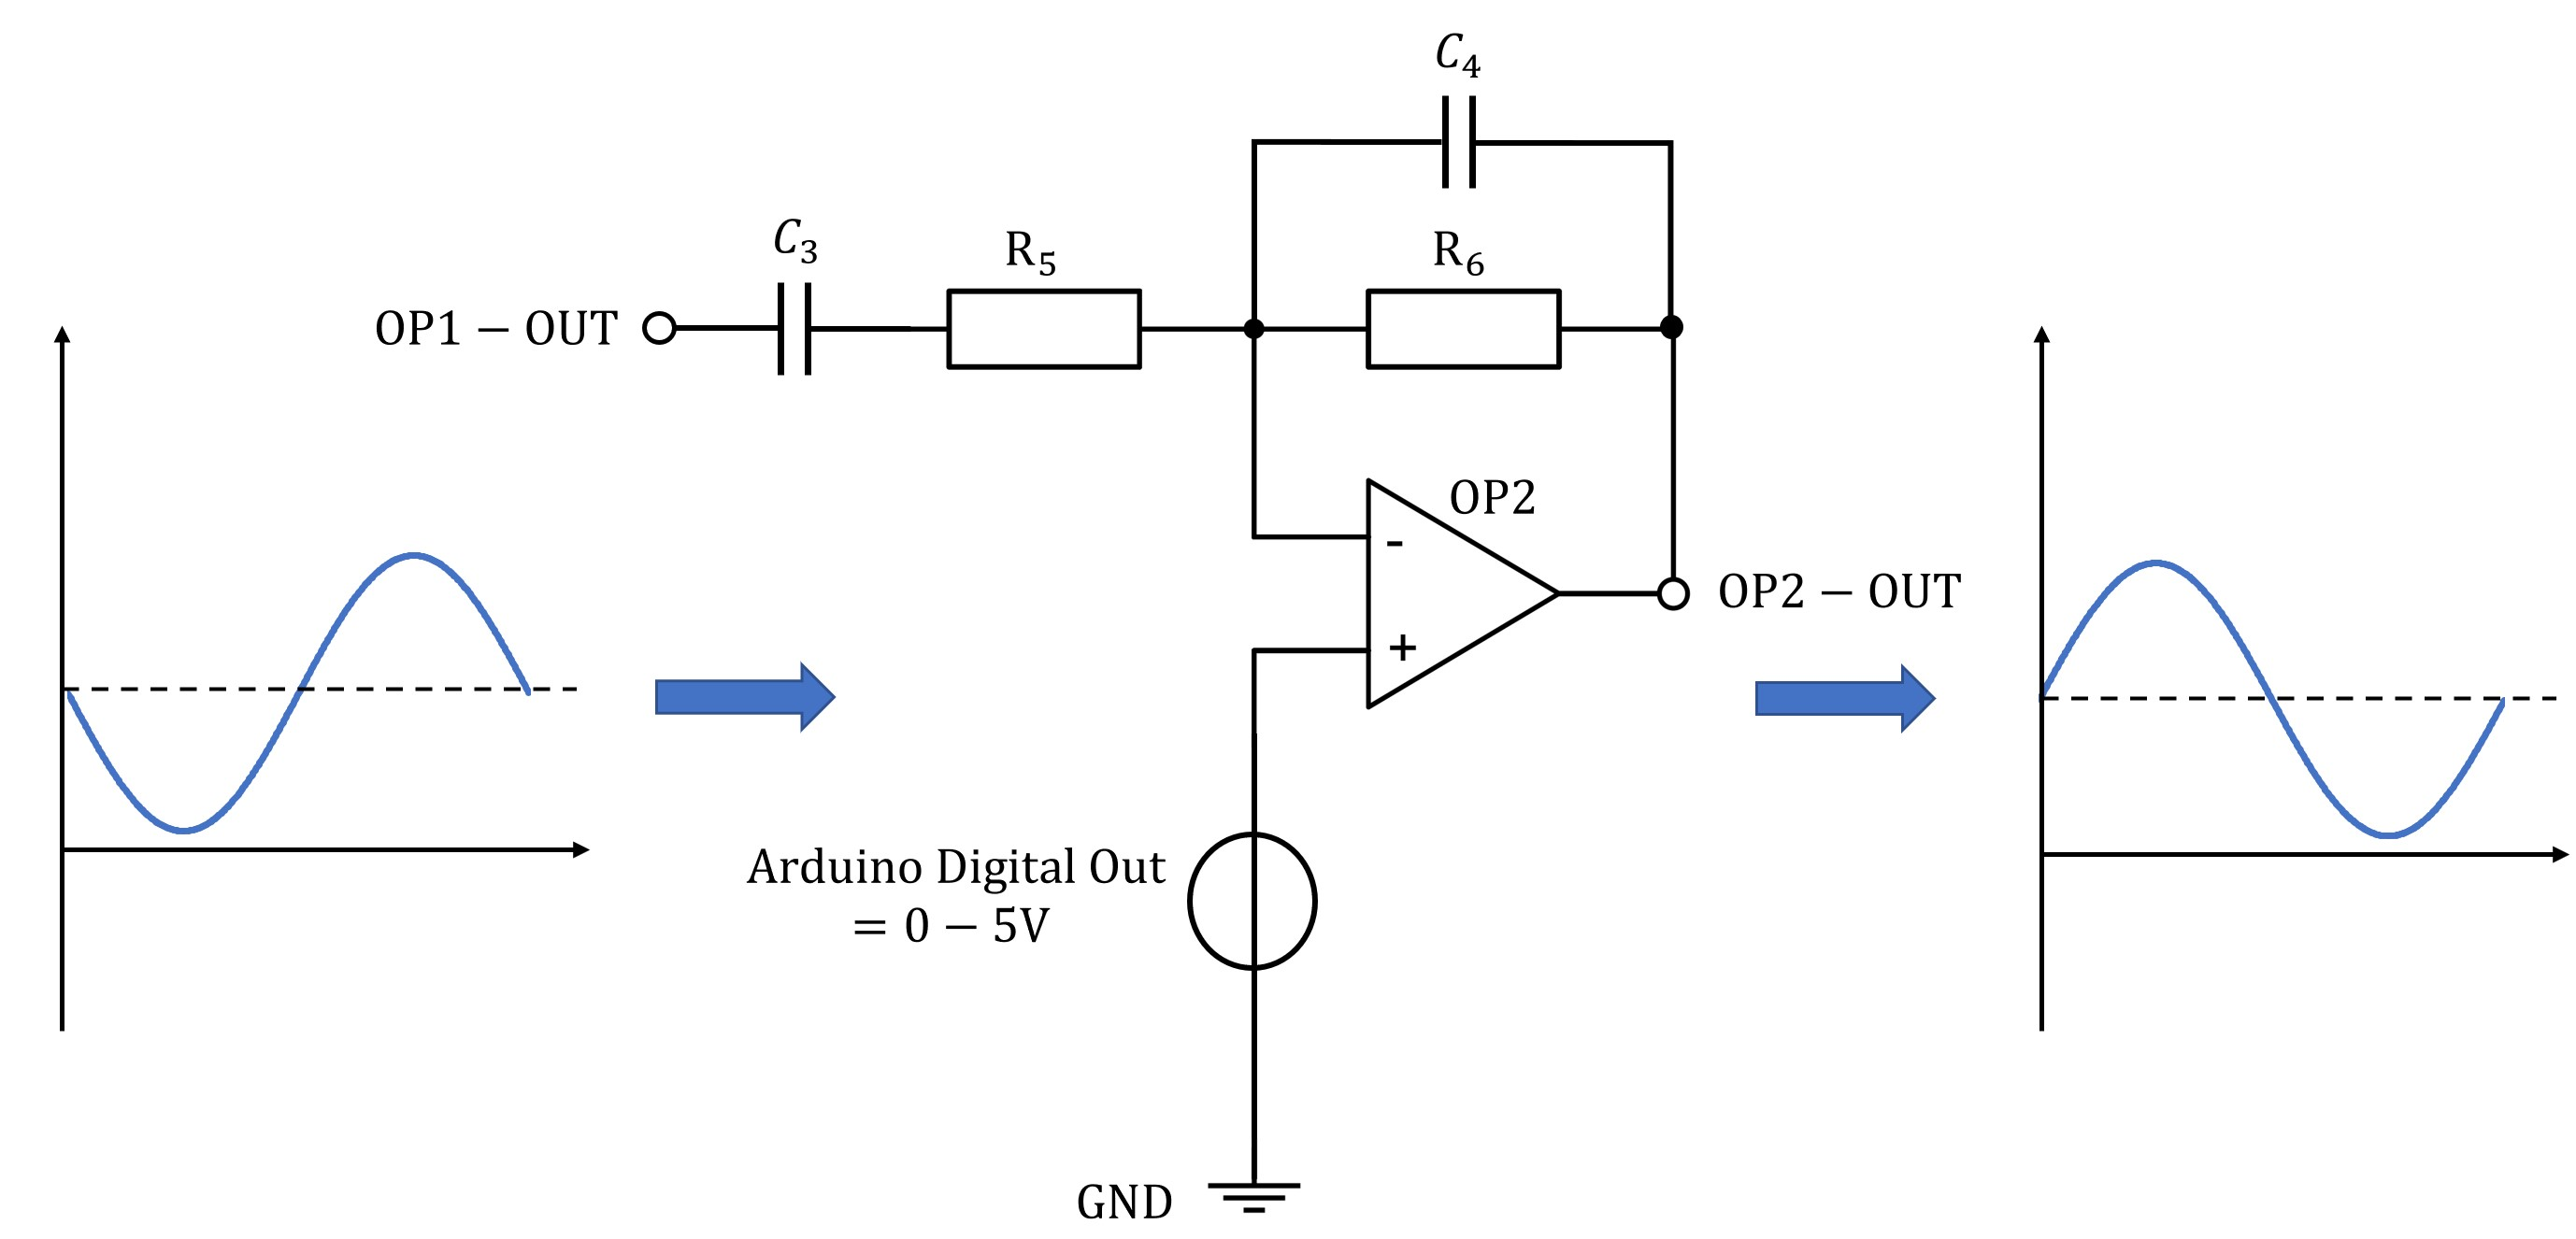
\includegraphics[width = 0.9 \textwidth ]{stufe2.jpg}
	\caption[Zweite Signalverarbeitungsstufe]{Zweite Signalverarbeitungsstufe} \gls{online:Eigen}
	\label{fig:stufe2}
\end{figure}


Die sehr hohe Vorwärtsverstärkung und die differentielle Eingangscharakteristik des \gls{acr:OP}s können genutzt werden, um eine nahezu ideale spannungsgesteuerte Stromquelle oder einen Spannungs-zu-Strom-Wandler zu realisieren. Es ist jedoch zu beachten, dass die umzuwandelnde Eingangsspannung an den nicht invertierenden Eingang des \gls{acr:OP}s angelegt wird. Der invertierende Eingang ist in Rückkopplung mit einem Ende des Widerstands $R{1}$ und der Source des Transistors $M{1}$ verbunden. Dies sorgt dafür, dass zwischen den Eingängen des \gls{acr:OP}s kein Spannungsunterschied herrscht. Der Ausgang des \gls{acr:OP}s steuert also das Gate des \gls{acr:MOSFET}s. Seine hohe Leerlaufverstärkung zwingt das Gate von $M{1}$ auf die erforderliche Spannung. Dadurch wird die Spannung, welche an $OP2-OUT = U_{R1}$ anliegt auf die Source des \gls{acr:MOSFET}s gespiegelt. Draus ergibt sich der Strom zu: 

\begin{equation}
	\label{equ:bsp1}
	I_{R1} = \frac{U_{R1}}{R_{1}}
\end{equation}

\begin{figure}[H]
	\centering
	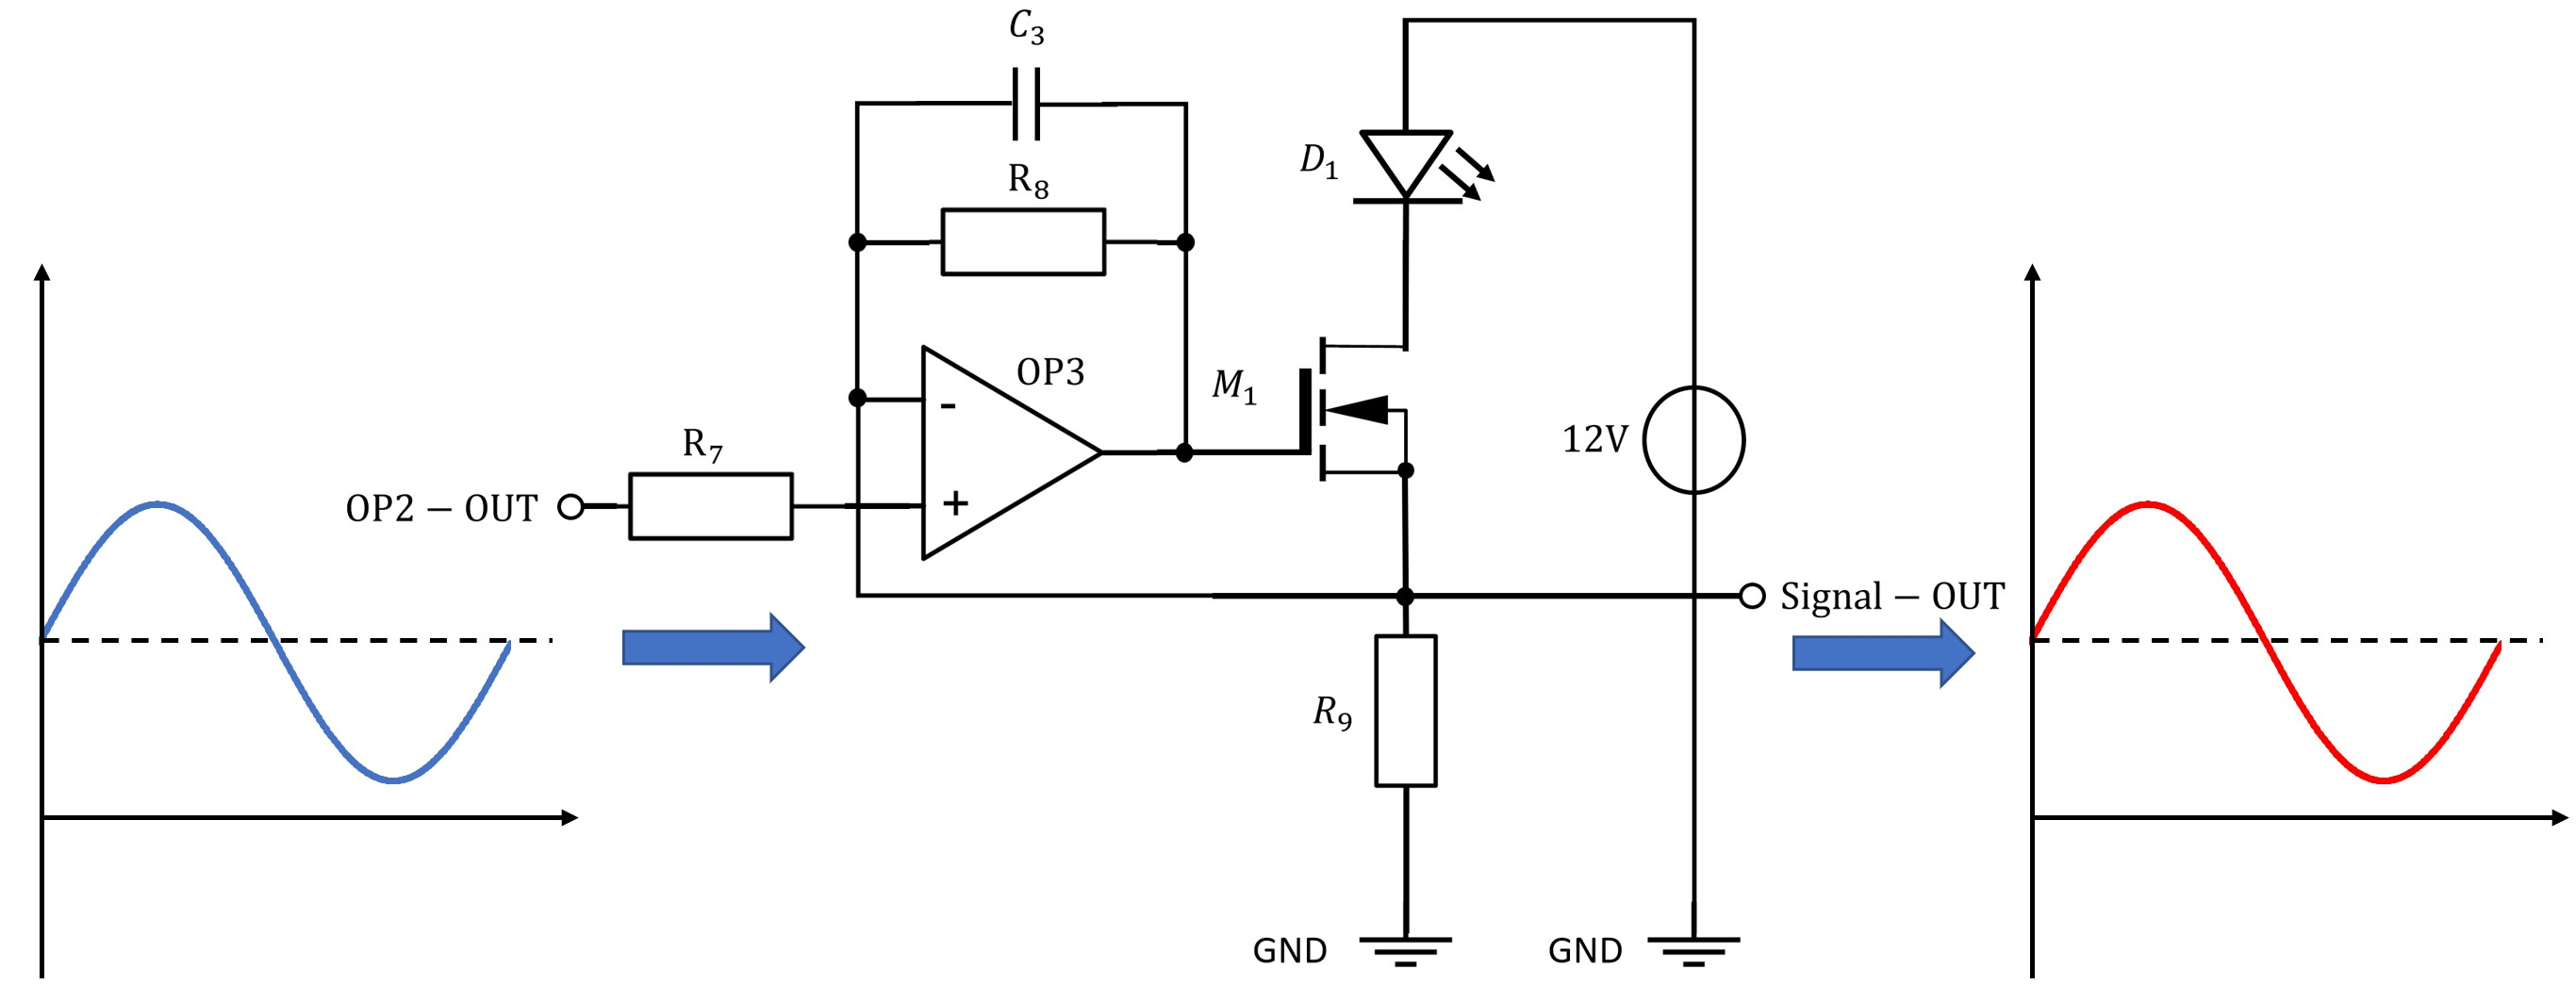
\includegraphics[width = 0.9 \textwidth ]{endstufe.jpg}
	\caption[LED- Treiber als Endstufe]{LED- Treiber als Endstufe} \gls{online:Eigen}
	\label{fig:endstufe}
\end{figure}

Durch die Bekanntheit des Stromflusses durch $R_1$ kann nun durch kirchhoffsche Regeln auf den Stromfluss in der \gls{acr:LED} geschlossen werden.\gls{online:vtoi} Dieser Strom wiederum erzeugt über selbigen Widerstand eine Anhebung des Potentials am - Eingang des \gls{acr:OP}s. Auf diese Weise versucht der \gls{acr:OP} seine beiden Eingänge auf das gleiche Potential anzuheben. Beim Leistungswiderstand $R_{9}$ handelt es sich um einen sehr kleinen Widerstand, weshalb durch die \gls{acr:LED}, den \gls{acr:MOSFET} und den Leistungswiderstand ein sehr hoher Strom fließt. Dieser sorgt für eine hell leuchtende \gls{acr:LED} zur Übertragung des Signals.

\subsection{Simulation in LT-Spice}
\label{subsec:Unterabschnitt1}

Das vorausgegangene theoretische Wissen wurde zudem mit einer LT-Spice Simulation überprüft. So konnten eventuelle Fehler bei der Dimensionierung ermittelt und verbessert werden werden. 

\begin{figure}[H]
	\centering
	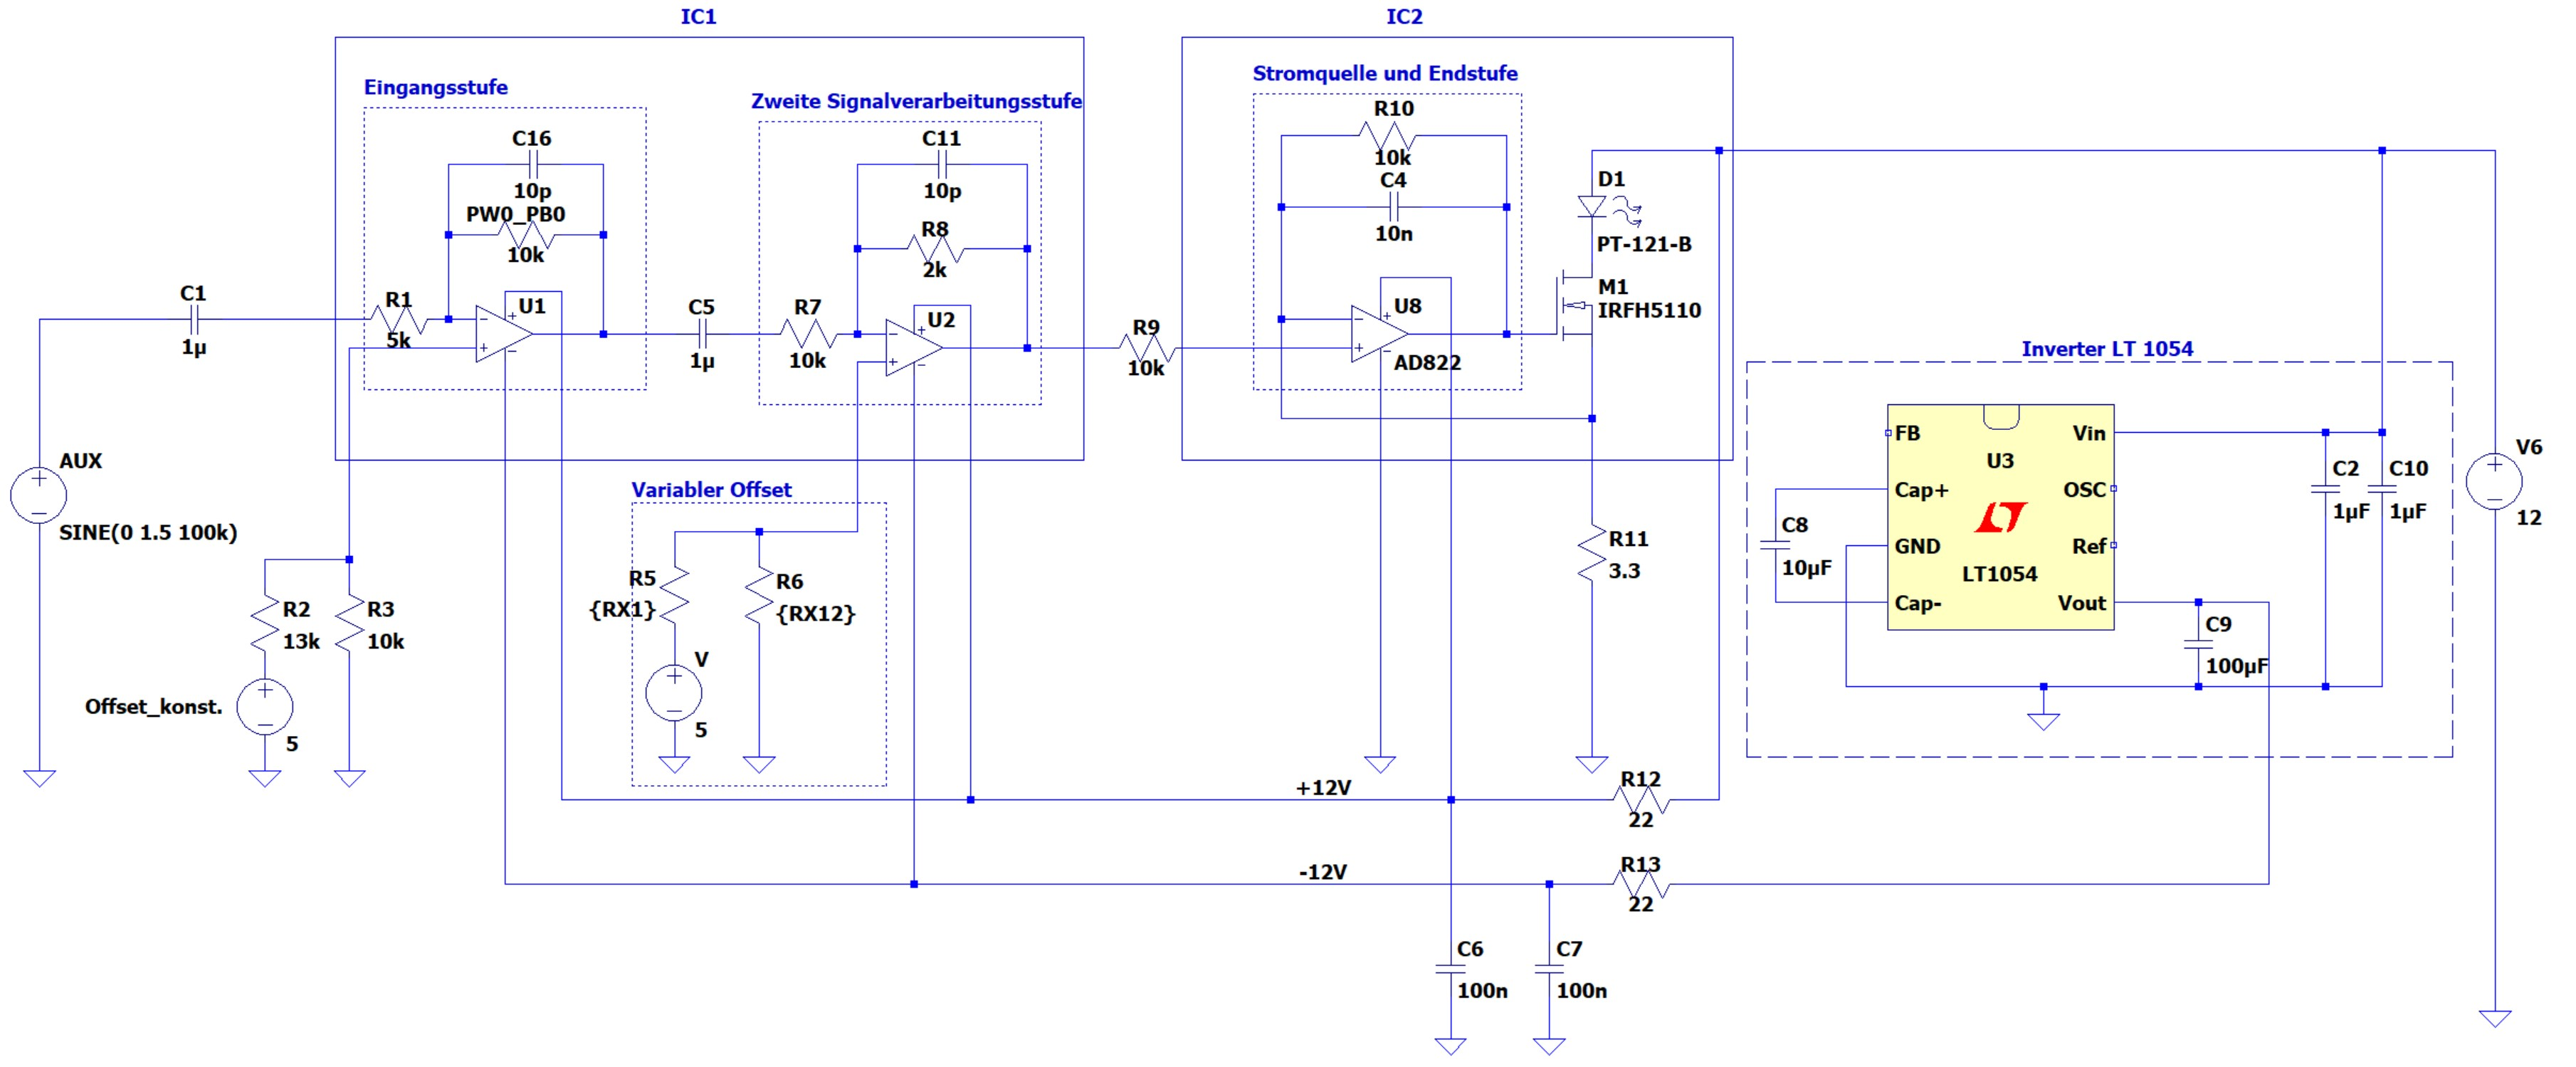
\includegraphics[width = 1 \textwidth ]{spice.jpg}
	\caption[LT-Spice Simulation der Signalverarbeitung]{LT-Spice Simulation der Signalverarbeitung} \gls{online:Eigen}
	\label{fig:spice}
\end{figure}

\subsection{Platinenlayout in Eagle}
\label{subsec:Unterabschnitt12}

Beim Platinenlayout Entwurf vom Senders wurde ein besonderes Augenmerk auf die Trennung von Signal und Leistungswegen geachtet.

\begin{figure}[H]
	\centering
	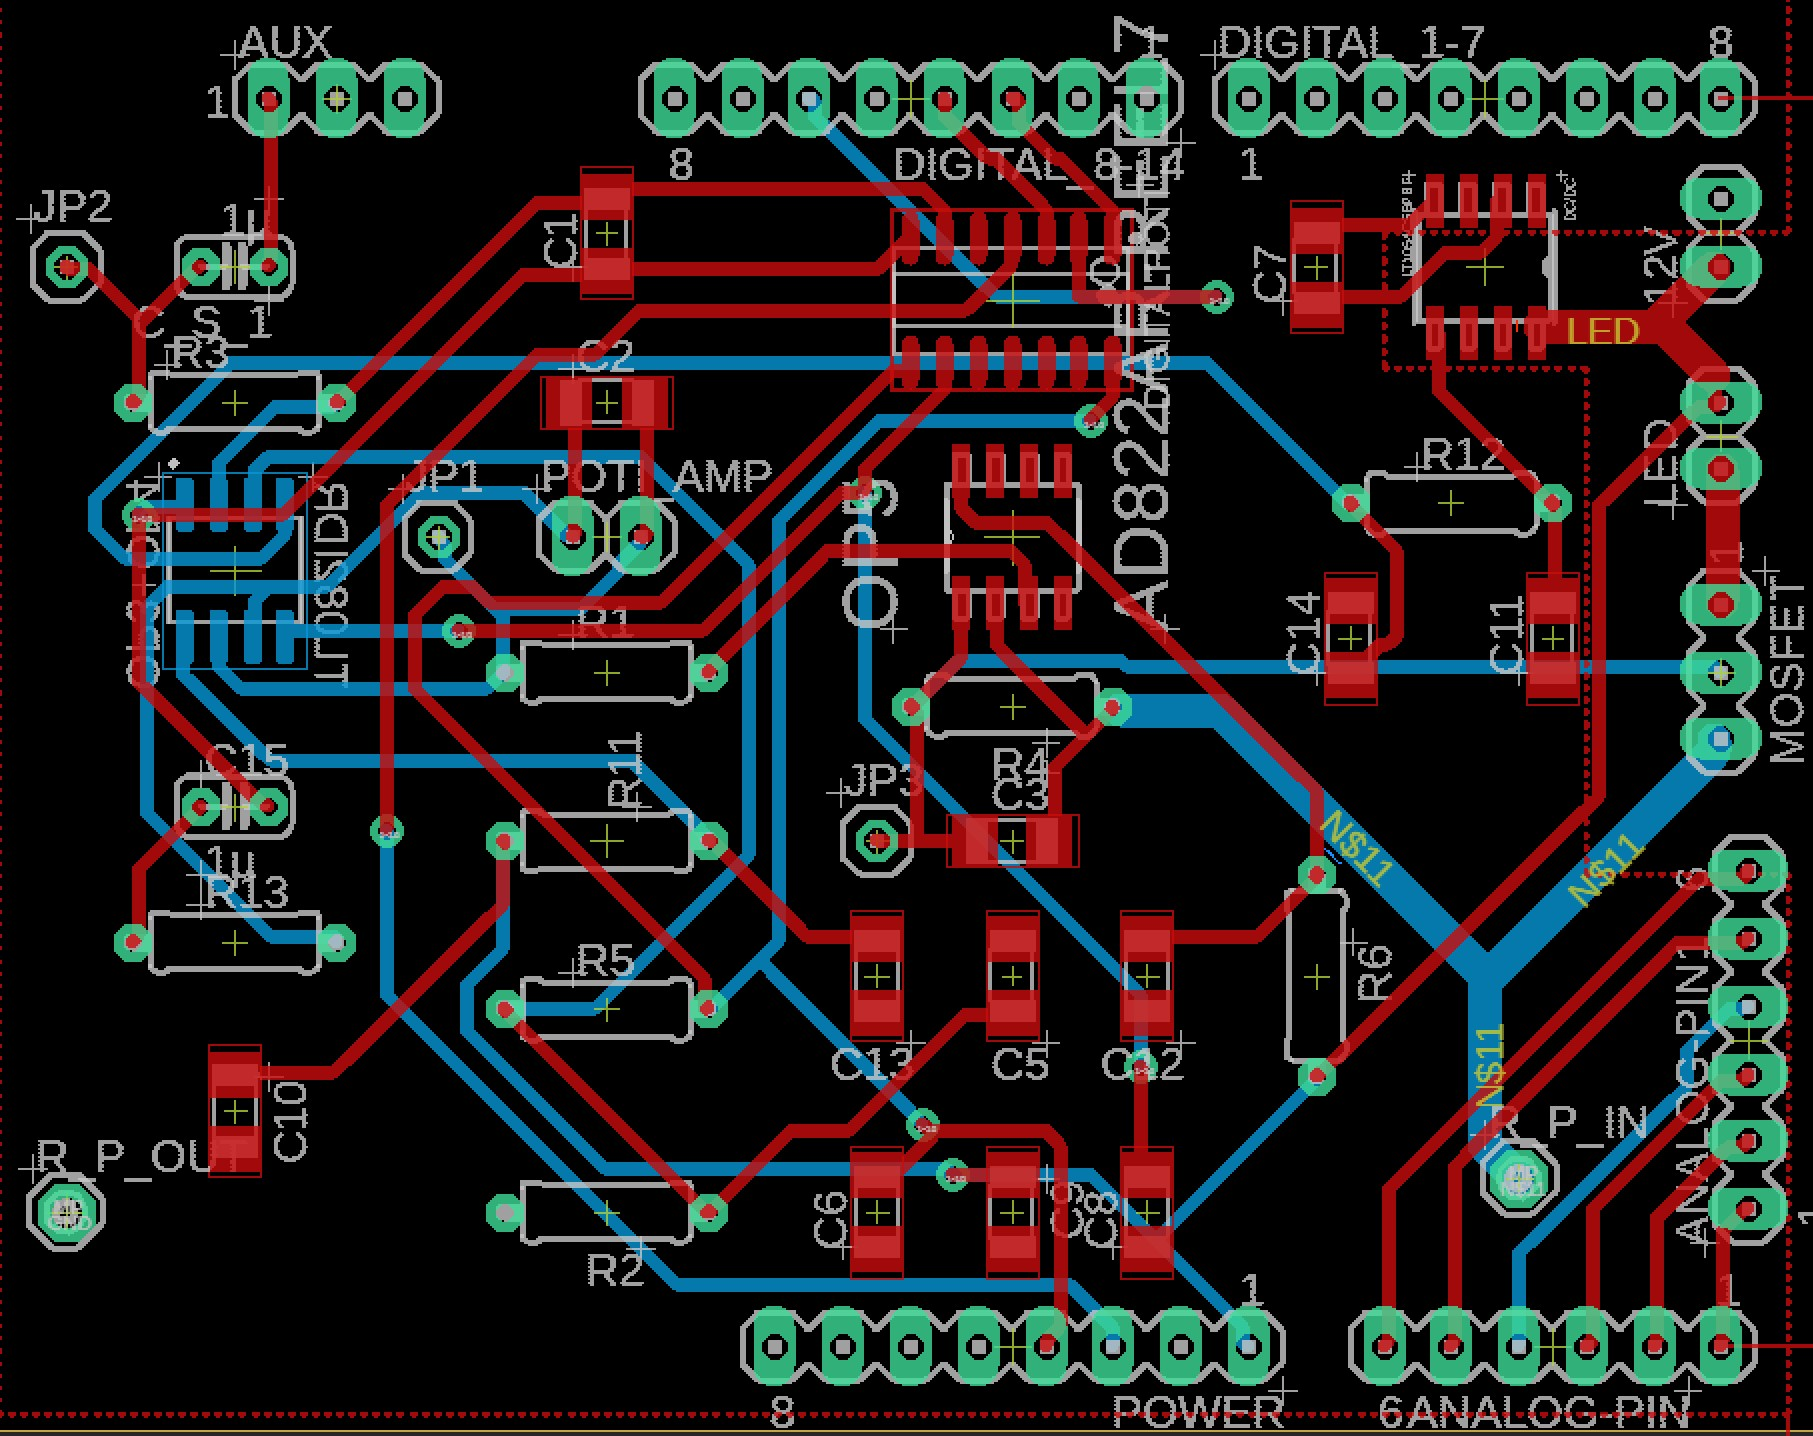
\includegraphics[width =0.8 \textwidth ]{eagle.jpg}
	\caption[Eagle Auszug der Platine]{Eagle Auszug der Platine} \gls{online:Eigen}
	\label{fig:eagle}
\end{figure}

Im unteren Bereich der Platine befindet sich der Leistungswiderstand, welcher sich von $R-P-IN$ zu $R-P-OUT$ erstreckt. Zuzüglich befinden sich der DC/DC Spannungswandler, \gls{acr:LED} und \gls{acr:MOSFET}, die signifikanten Bauteile der Stromquelle auf des Rechten Seite der Platine und somit möglichst weit vom Signalverarbeitungspfad entfernt. In der Schaltung fließen teilweise Ströme bis 1,35A. Da es bei solch hohen Strömen zu Problemen mit der   \gls{acr:EMV} kommen kann, wurde der Signalweg linksseitig auf der Platine positioniert. Außerdem wurden die Leiterbahnen im Leistungspfad besonders breit ausgelegt, da hier große Ströme fließen. Genaue Informationen über die Dimensionierung der Leiterbahnen und Abstände ist in Tabelle~\ref{tab:leiterbahnen} zu finden. Auf der Platine wurden für die Operationsverstärker, das Digitalpotentiometer und den DC/DC Spannungswandler IC-Sockel aufgelötet. Das ermöglicht den schnellen Austausch von defekten Bauteilen. Die komplette Schaltung des \gls{acr:VLC}-Senders wurde auf die Größe einer kleinen gefrästen Platine untergebracht. Deshalb wurden Leitungen auf der Rückseite der Platine verlegt. Diese sind in Abbildung ~\ref{fig:eagle} durch die Blauen Leiterbahnen dargestellt. Des weiteren wurden im Signalverarbeitungspfad nach jeder Stufe Pins vorgesehen, um die Fehlersuche zu erleichtern und nachträglich einzelne Funktionsprüfungen durchzuführen. Hinzu ist zu beachten, dass die Bauteile im Leistungspfad durch den hohen Stromfluss eine hohe thermische Abgabe an Energie verzeichnen müssen. Um diese zu reduzieren wurden Kühlkörper vorgesehen. Wie diese Berechnet und Dimensioniert werden wird in Kapitel ~\ref{subsub:thermo} näher erläutert. Um die Schaltung zuletzt noch zusätzlich weniger Störanfällig zu gestalten, wurden die gegebenen freien Flächen auf beiden Seiten der Platine mit dem Masse Potential ausgefüllt. 

\subsection{Thermisches Management}
\label{subsub:thermo}
Wie im vorherigen Kapitel schon erwähnt, fließt durch den Leistungsstrang der Schaltung ein sehr hoher Strom. Durch diesen hohen Stromfluss kommt es zu einer immensen Hitzeentwicklung in den Bauteilen. Um jedoch die einwandfreie Funktion von elektronischen Halbleiterbauelementen zu gewährleisten, ist die Einhaltung der vom Hersteller angegebenen maximalen Sperrschichttemperaturen unerlässlich. Solch eine Sperrschichttemperatur lässt sich nur bei geringer Leistungsanforderung ohne Kühlung einhalten. Zudem sind die Einbaulage, der Einbauort, die Geschwindigkeit und Temperatur der Umgebungsluft variable Größen die miteinzukalkulieren sind.\gls{online:thermo}

\begin{figure}[H]
	\centering
	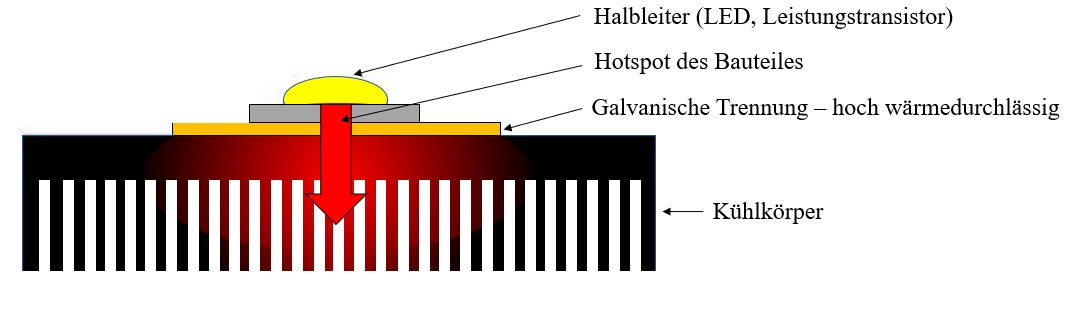
\includegraphics[width =1 \textwidth ]{thermo.jpg}
	\caption[Montageschema eines Kühlkörpers]{Montageschema eines Kühlkörpers} \gls{online:Eigen}\gls{online:thermo2}
	\label{fig:thermo}
\end{figure}

Um gegen diese Hitzeentwicklung vorzugehen wird für die kritischen Bauteile somit ein Kühlkörper vorgesehen. Diese sollen die Wärme vom Bauteil weg und nach außen hin abführen. In dem hier gegebenen elektrischen Stromkreis, werden zwei Halbleiter als kritische und zu kühlende Bauteile betrachtet. Zunächst die \gls{acr:LED} zum Übertragen des Signals und zum zweiten der \gls{acr:MOSFET}.\cite{thermLED}

Zur Auswahl eines geeigneten Kühlkörpers für ein Halbleiterbauelement ist die Berechnung des Wärmewiderstandes unerlässlich. Dafür werden die in Tabelle~\ref{tab:thermofaktoren} aufgeführten Variablen in folgende Gleichung eingesetzt.

\begin{equation}
	\label{equ:thermo}
	R_{thK} = \frac{\vartheta_{i}-\vartheta_{u}}{P}-(R_{thG}+R_{RthM})
\end{equation}

\begin{table}[htb]
	\begin{center}
		\begin{tabular}[h]{c|l}	
			
			Faktor & Bedeutung \\
			\hline
			$\vartheta_{i}$& Herstellerangabe der Halbleiters zur max. Sperrschichttemperatur\\
			$\vartheta_{u}$& Umgebungstemperatur in $^\circ C$ \\
			$P$ &  Die am zu kühlenden Halbleiter maximal anfallende Leistung in Watt\\
			Rth & Wärmewiderstand allgemein in $\frac{K}{W}$ \\
			RthG & Herstellerangabe zum innerer Wärmewiderstand des Halbleiters \\
			RthM & Wärmewiderstand der Montagefläche \\
			RthK &  Wärmewiderstand des Kühlkörpers \\
			
		\end{tabular}
		\caption{Variablen zu berechnung des Kühlkörpers}\gls{online:thermo1}
		\label{tab:thermofaktoren}
	\end{center}
\end{table}

Für die Berechnung der Kühlkörper wurden zudem Berechnungen zur Verlustleistung des
\gls{acr:MOSFET}s und der \gls{acr:LED} vorgenommen. Es wird bewusst überdimensioniert. Dazu wurde beispielsweise für die \gls{acr:LED} mit einem Wirkungsgrad von 0 \% gerechnet. Unter diesen Umständen würde die Verlustleistung 100 \% betragen. \gls{acr:LED}s haben jedoch tatsächlich einen Wirkungsgrad von ca. 25 - 50 \%. Die maximalen Verluste werden natürlich bei voller Helligkeit verzeichnet. Zur Auslegung der Kühlkörper wurden also folgende Berechnungen durchgeführt:

\begin{equation}
	\label{equ:thermoled}
	P_{LED} = U_{LED} \cdot I_{G} = 3,12V \cdot 1,42A= 4,43W
\end{equation}

\begin{equation}
	\label{equ:thermomos}
	P_{MOSFET} = U_{MOSFET} \cdot I_{G} = 4,1V \cdot 1,42A= 5,86W
\end{equation}

Wodurch sich der Wärmewiderstand der Kühlkörper für die \gls{acr:LED} zu

\begin{equation}
	\label{equ:thermo2}
	R_{thK-LED} = \frac{35 ^\circ C - 25 ^\circ C}{4,43W}-(1 \frac{^\circ C}{W}+0,1 \frac{^\circ C}{W}) = 1,36\frac{^\circ C}{W}
\end{equation}

berechnet und der Wärmewiderstand des \gls{acr:MOSFET} aus
 
\begin{equation}
	\label{equ:thermo3}
	R_{thK-MOSFET} = \frac{50 ^\circ C - 25 ^\circ C}{5,86W}-(1,15 \frac{^\circ C}{W}+0,1 \frac{^\circ C}{W}) = 3,22\frac{^\circ C}{W}
\end{equation}
ergibt. Gewählt wurde zuletzt für sowohl \gls{acr:LED} als auch \gls{acr:MOSFET} ein Kühlkörper in der Größenordnung von 3 $^\circ C/W$.


\subsection{Planung und Aufbau des Gehäuses}
\label{subsec:Unterabschnitt12}

\begin{figure}[H]
	\centering
	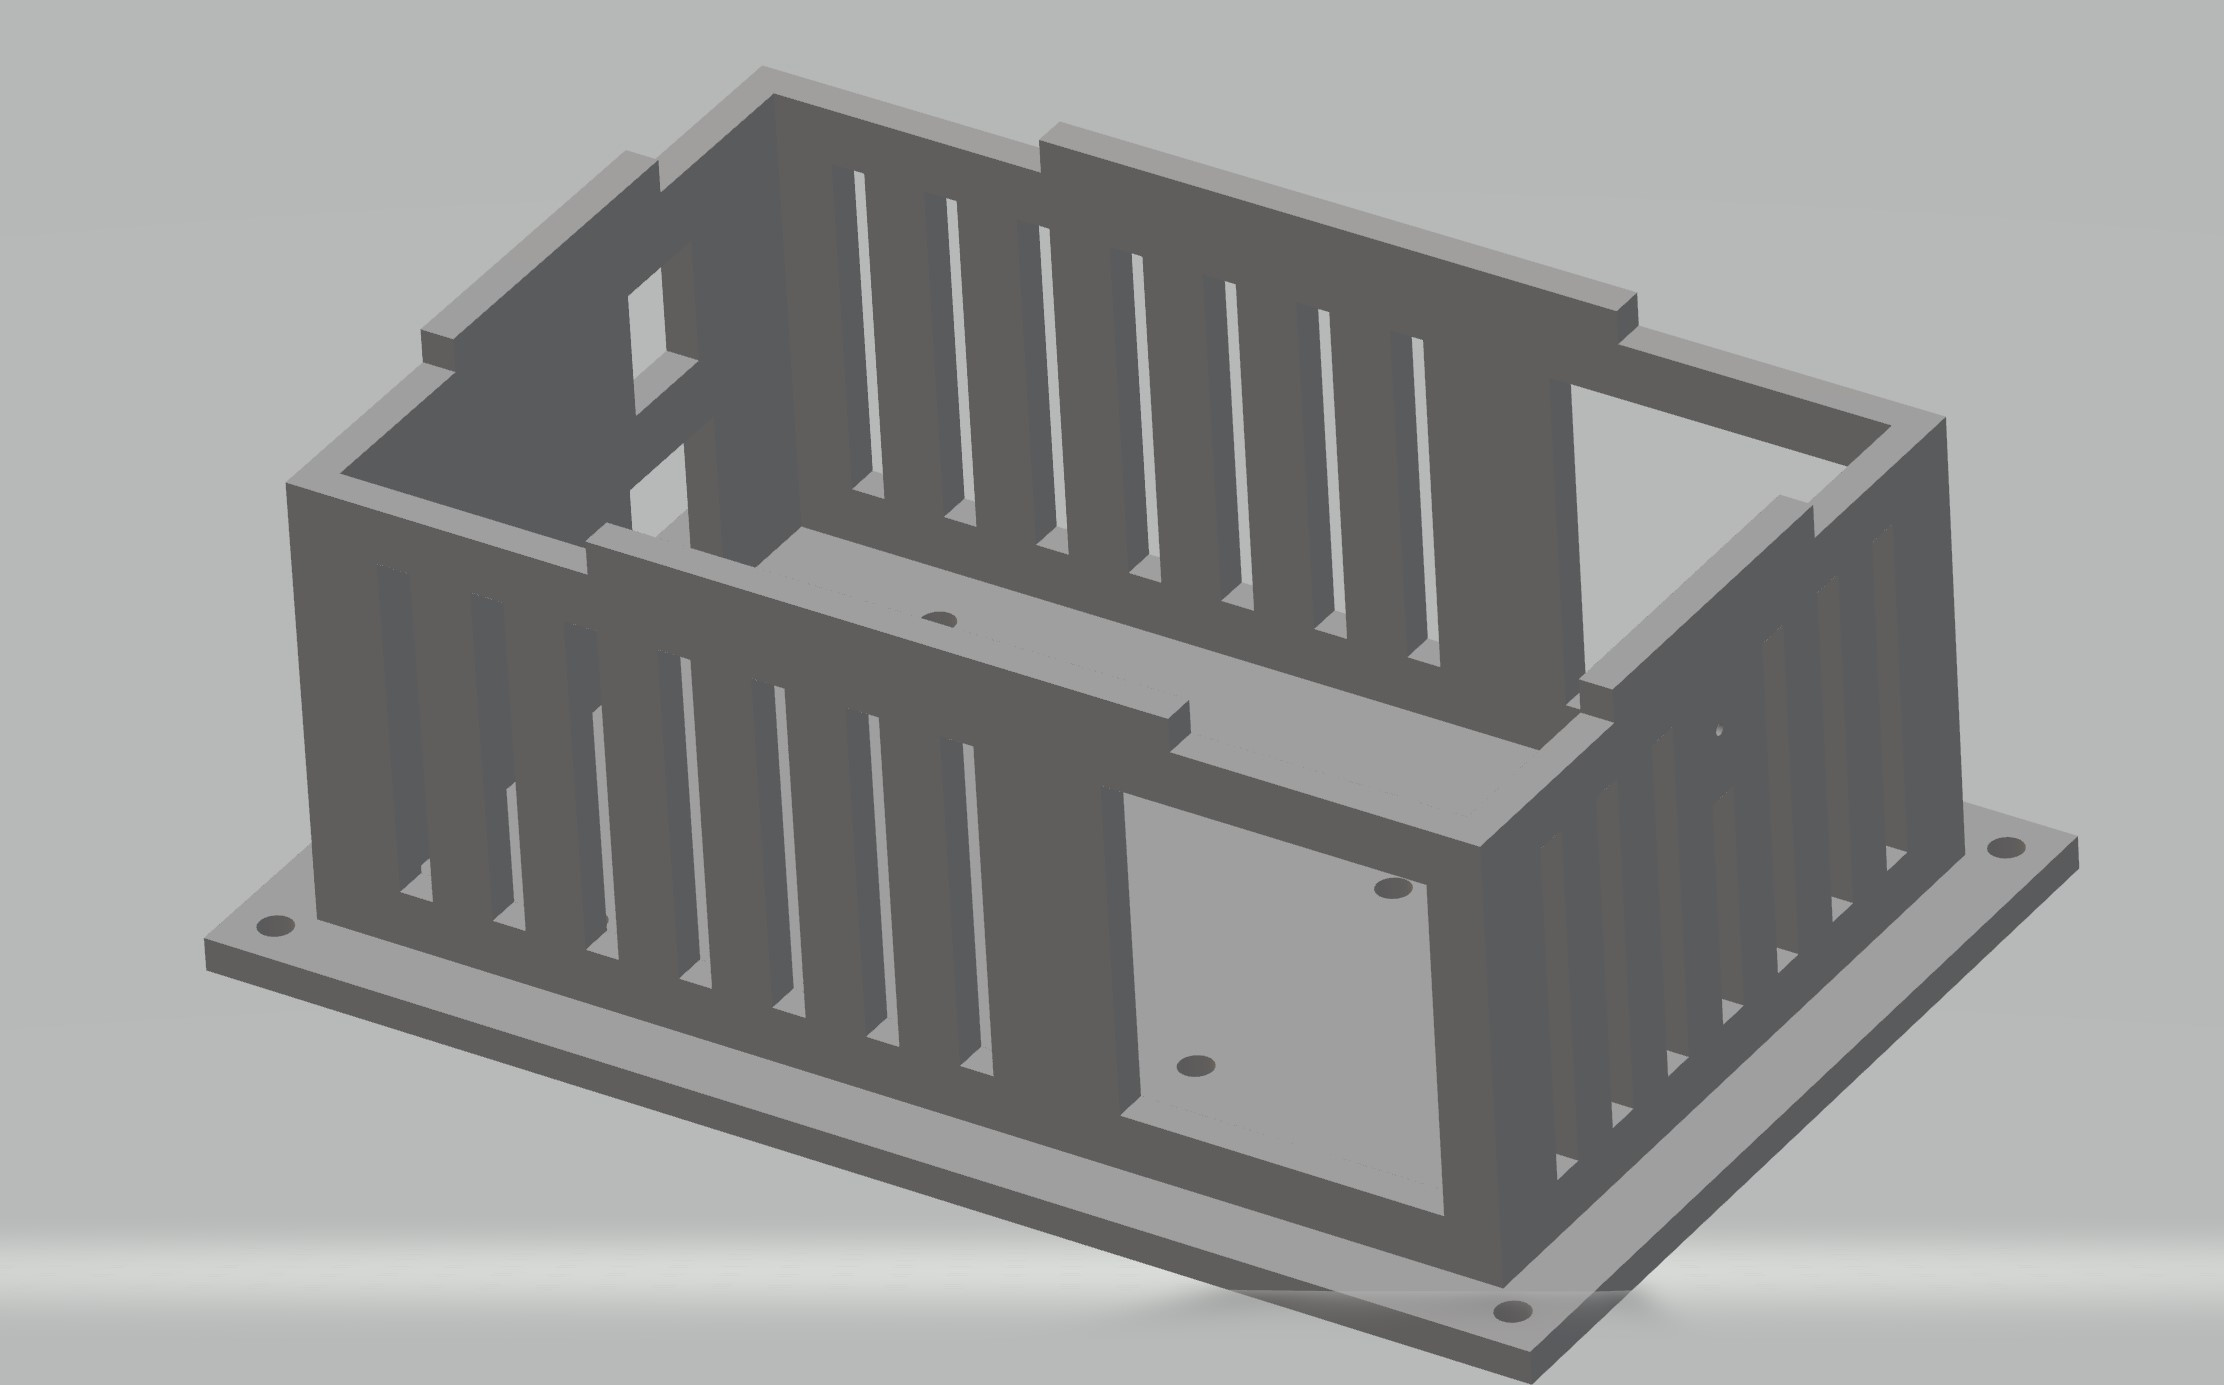
\includegraphics[width =1 \textwidth ]{3dbottom.jpg}
	\caption[Boden des 3D-Drucks]{Boden des 3D-Drucks} \gls{online:Eigen}
	\label{fig:3dbottom}
\end{figure}

Beim Entwurf des Gehäuses wurde so Platzsparend wie möglich gearbeitet, weshalb
der fest verbaute Arduino zwischen Leiterplatte und Deckel angebracht wurde.
Da sich Leistungswiderstand, Transistor und Leuchtdiode im Betrieb stark erhitzen,
wurden die zugehörigen Kühlkörper am Boden mithilfe von Abstandsbolzen
befestigt. Zusätzlich wurden im Deckel Freischnitte über den Kühlkörpern vorgenommen
um die nach oben steigende Luft möglichst gut abzuleiten. Für die
Versorgungsspannung der Schaltung gibt es zwei 4mm Anschlüsse, die oben am
Deckel angebracht wurden. Für die Datenübertragung wurde eine AUX Buchse im
Deckel verbaut.

\section{Software}
\label{sec:Software}
\subsection{Automatisierte Amplituden-Regelung}
\label{subsec:Unterabschnitt12}


\subsection{Übertragung mit Dream}
\label{subsec:dream}

Das Programm verfügt auf zwei verschiedene Möglichkeiten aufgerufen werden. Zum ersten im Sendemodus und zum zweiten im Empfangsmodus. Zudem bietet Dream umfangreiche Einstellungsoptionen um sowohl Rauschen oder aber auch andere Störungen zu minimieren. Die wichtigsten Parameter für die Korrekte Benutzung werden in dend
folgenden zwei Kapiteln näher erläutert.



\subsubsection{Dream Transmitter}
\label{subsubsec:dreamtx}
Zum Start der Software ”Dream” im Übertragungsmodus muss das Programm mit dem parameter ”- t” gestartet werden. Die einfachste Möglichkeit für einen Programmstart mit Parameter bietet eine Verknüpfung, welche wie in Abbildung 15 gezeigt, angepasst wird. Das Zielverzeichnis darf dabei nicht verändert werden! Dieser Schritt muss nur einmal gemacht werden und man kann jederzeit den Übertragungsmodus starten indem man die Dream software über diese geänderte Verknüpfung startet.

\begin{figure}[H]
	\centering
	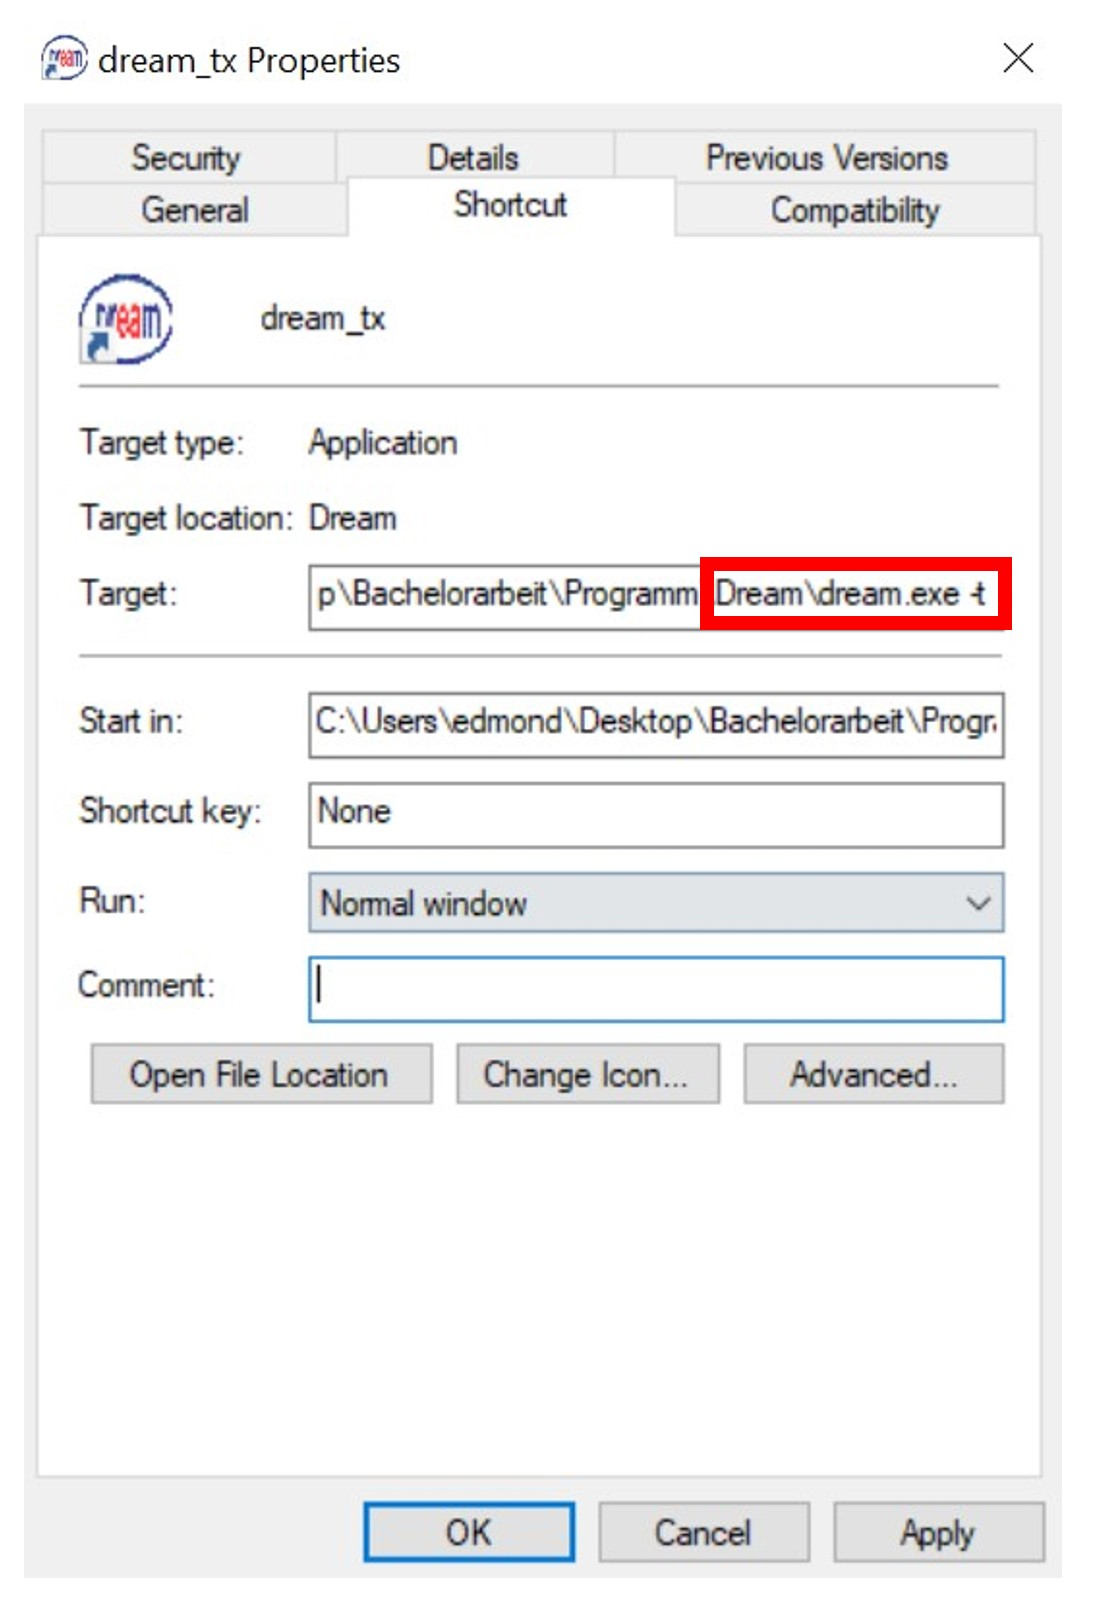
\includegraphics[width = 0.5 \textwidth ]{dreamtx.jpg}
	\caption[Modifizierung für den Sendemodus]{Modifizierung für den Sendemodus} \gls{online:Eigen}
	\label{fig:dreamtx}
\end{figure}

\begin{figure}[H]
	\centering
	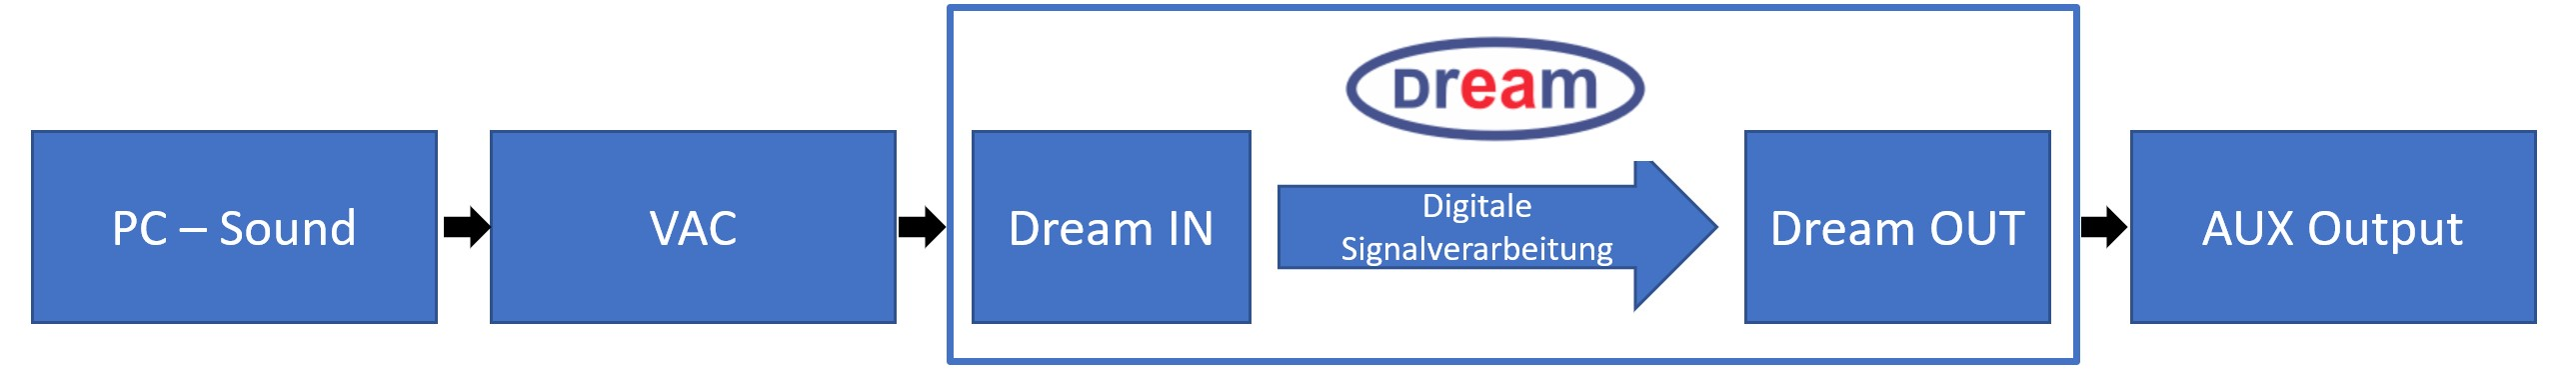
\includegraphics[width = 0.9 \textwidth ]{dreamtxeinstellung.jpg}
	\caption[Internes Audiorouting]{Internes Audiorouting} \gls{online:Eigen}
	\label{fig:dreamtxeinstellung}
\end{figure}

\subsubsection{Dream Receiver}
\label{subsec:Unterabschnitt12}

Der Evaluation Dialog liefert detaillierte Informationen über die empfangenen DRM-Parameter. Hier können Parameter sowie einige Diagramme eingesehen werden. In den folgenden Tabellen, werden für die Übertragung bedeutende Parameter näher erläutert.

\begin{table}[h]
	\begin{center}
		\begin{tabular}{p{0.3\linewidth} | p{0.7 \linewidth}}	
			\textbf{Measurements} & \\
			\hline
			\textbf{DC Frequency Offset} & Dieser Offset entspricht der resultierenden Soundkarten-Zwischenfrequenz des Frontends. Diese Frequenz ist nicht auf einen bestimmten Wert beschränkt, sondern nur darauf, dass das DRM-Spektrum vollständig innerhalb der Bandbreite der Soundkarte liegen muss.\\
			
			\textbf{Sample Frequency Offset} & Offset der Abtastrate des lokalen Computers zum DA-Wandler im Sender. \\
			
			\textbf{Doppler / Delay} & The Doppler frequency of the channel is estimated for the Wiener filter design of channel estimation in time direction. If linear interpolation is set for channel estimation in time direction, this estimation is not updated. The Doppler frequency is an indication of how fast the channel varies with time. The higher the frequency, the faster the channel changes are.
			The total delay time of the Power Delay Spectrum (PDS) is estimated from the impulse response estimation derived from the channel estimation. This delay corresponds to the range between the two vertical dashed black lines in the Impulse Response (IR) plot. \\
			\textbf{I/O Interface LED} & This LED shows the current status of the sound card interface. The yellow light shows that the audio output was corrected. Since the sample rate of the transmitter and local computer are different, from time to time the audio buffers will overflow or under run and a correction is necessary. When a correction occurs, a "click" sound can be heard. The red light shows that a buffer was lost in the sound card input stream. This can happen if a thread with a higher priority is at 100 and the Dream software cannot read the provided blocks fast enough. In this case the Dream software will instantly loose the synchronization and has to re-synchronize. Another reason for red light is that the processor is to slow for running the Dream software.
			\\
			\textbf{Time Sync Acq LED} & This LED shows the state of the timing acquisition (search for the beginning of an OFDM symbol). If the acquisition is done, this LED will stay green.
			\\
			\textbf{Frame Sync LED} & The DRM frame synchronization status is shown with this LED. This LED is also only active during acquisition state of the Dream receiver. In tracking mode this LED is always green.
			\\
			\textbf{FAC CRC LED} & This LED shows the Cyclic Redundancy Check (CRC) of the Fast Access Channel (FAC) of DRM. FAC is one of the three logical channels and is always modulated with a 4-QAM. If the FAC CRC check was successful, the receiver changes to tracking mode. The FAC LED is the indication whether the receiver is synchronized to a DRM transmission or not. \\
			\textbf{SRC CRC LED} & 	This LED shows the CRC check result of the Service Description Channel (SDC) which is one logical channel of the DRM stream. This data is transmitted in approx. 1 second intervals and contains information about station label, audio and data format etc. The error protection is normally lower than the protection of the FAC. Therefore this LED will turn to red earlier than the FAC LED in general. \\
			\textbf{MSC CRC LED} & This LED shows the status of the Main Service Channel (MSC). This channel contains the actual audio and data bits. The LED shows the CRC check of the AAC core decoder. The SBR has a separate CRC, but this status is not shown with this LED. If SBR CRC is wrong but the AAC CRC is ok one can still hear something (of course, the high frequencies are not there in this case). If this LED turns red, interruptions of the audio are heard. The yellow light shows that only one 40 ms audio frame CRC was wrong. This causes usually no hearable artifacts.\\
			
			
			
			
			
			\hline
		\end{tabular}
		\caption{Unterschrift  der Tabelle}
		\label{tab:Tabelle1}
	\end{center}
\end{table}

\begin{table}[h]
	\begin{center}
		\begin{tabular}{p{0.3\linewidth} | p{0.7\linewidth}}	
			
			\textbf{Parameters} &  \\
			\hline
			\textbf{DRM mode/ bandwidth} & In a DRM system, four possible robustness modes are defined to adapt the system to different channel conditions. According to the DRM standard:\newline
			\textbf{Mode A}: Gaussian channels, with minor fading\newline
			\textbf{Mode B}: Time and frequency selective channels, with longer delay spread\newline
			\textbf{Mode C}: As robustness mode B, but with higher Doppler spread\newline
			\textbf{Mode D}: As robustness mode B, but with severe delay and Doppler spread\newline
			The bandwidth is the gross bandwidth of the current DRM signal. \\
			\textbf{Interleaver Depth} & The symbol interleaver depth can be either short (approx. 400 ms) or long (approx. 2 s). The longer the interleaver the better the channel decoder can correct errors from slow fading signals. But the longer the interleaver length the longer the delay until audio can be heard (after a re-synchronization).
			\\
			\textbf{SDC / MSC Mode} & Shows the modulation type of the SDC and MSC channel. For the MSC channel, some hierarchical modes are defined which can provide a very strong protected service channel.
			\\
			\textbf{Prot. Level (B/A)} & The error protection level of the channel coder. For 64-QAM, there are four protection levels defined in the DRM standard. Protection level 0 has the highest protection whereas level 3 has the lowest protection. The letters A and B are the names of the higher and lower protected parts of a DRM block when Unequal Error Protection (UEP) is used. If Equal Error Protection (EEP) is used, only the protection level of part B is valid.
			\\
			\textbf{Number of Services} & This shows the number of audio and data services transmitted in the DRM stream. The maximum number of streams is four.
			\\
			\textbf{Received time - date} & This label shows the received time and date in UTC. This information is carried in the SDC channel.
			\\
			\hline
		\end{tabular}
		\caption{Unterschrift  der Tabelle}
		\label{tab:Tabelle1}
	\end{center}
\end{table}
\begin{table}[ht]
	\begin{center}
		\begin{tabular}{p{0.3\linewidth} | p{0.7\linewidth}}
			\textbf{Chart} & \\
			\hline
			\textbf{SNR} & Signal to Noise Ratio (SNR) estimation is plotted as a bar and as a value.
			\\
			\textbf{Main Plot} & Graphical display of different vectors of the DRM decoder. \\
			\hline
		\end{tabular}
		\caption{Unterschrift  der Tabelle}
		\label{tab:Tabelle1}
	\end{center}
\end{table}

\begin{table}[htb]
	\begin{center}
		\begin{tabular}{p{0.25\linewidth} | p{0.75\linewidth}}	
			
			\textbf{Advanced Settings} &  \\
			\hline
			\textbf{Frequency Interpolation} & With these settings the channel estimation method in frequency direction can be selected. The default value uses the most powerful algorithm.
			Wiener (default) - Wiener interpolation uses estimation of the statistics of the channel to design an optimal filter for noise reduction.
			Linear - Simple linear interpolation method to get the channel estimate. The real and imaginary parts of the estimated channel at the pilot positions are linearly interpolated. This algorithm causes the lowest CPU load but performs much worse than the Wiener interpolation at low SNR's.
			DFT Zero Pad: - Channel estimation method for the frequency direction using Discrete Fourier Transformation (DFT) to transform the channel estimation at the pilot positions to the time domain. A zero padding is applied to get a higher resolution in the frequency domain -> estimates at the data cells. This algorithm is very speed efficient but has problems at the edges of the OFDM spectrum due to the leakage effect. \\
			\textbf{Time Interpolation} & With these settings the channel estimation method in time direction can be selected. The default value uses the most powerful algorithm.
			Wiener (default) - Wiener interpolation uses estimation of the statistics of the channel to design an optimal filter for noise reduction.
			Linear - Simple linear interpolation method to get the channel estimate. The real and imaginary parts of the estimated channel at the pilot positions are interpolated linearly. This algorithm causes the lowest CPU load and the audio is decoded more quickly, but in general it performs worse than the Wiener interpolation especially at low SNR's. \\
			
			\textbf{Time Sync Tracking} & 	With these settings the time synchronization tracking methods can be selected.
			Guard Energy (default) - This algorithm utilizes the estimation of the impulse response and tries to maximize the energy in the guard-interval to set the correct timing.
			First Peak - This algorithm searches for the first peak in the estimated impulse response and moves this peak to the beginning of the guard-interval (timing tracking algorithm) \\
			
			\textbf{Flip Input Spectrum} & Checking this box will flip or invert the input spectrum. This is necessary if the mixer in the front-end uses the lower side band.
			\\
			
			\textbf{Mute Audio} & The audio can be muted by checking this box. The reaction of checking or unchecking this box is delayed by approx. 1 second due to the audio buffers.
			\\
			
			\textbf{MLC, Number of Iterations} & In DRM a multilevel channel coder is used. With this code it is possible to iterate the decoding process in the decoder to improve the decoding result. The more iterations are used the better the result will be. But switching to more iterations will increase the CPU load. Simulations showed that the first iteration (number of iterations = 1) gives the most improvement (approx. 1.5 dB at a BER of 10-4 on a Gaussian channel, Mode A, 10 kHz bandwidth). The improvement of the second iteration (number of iterations = 2) will be as small as 0.3 dB.
			The recommended number of iterations given in the DRM standard is one iteration (default value: number of iterations = 1).
			The selection is saved in the Dream.ini file. \\
			
			\textbf{Log File} & Checking this box causes Dream to write two kinds of log files about the current reception of an audio service using AAC source coding, a standard and a long log file. Both files are written to the directory were the Dream application is located.
			The standard log file DreamLog.txt is compatible to the log file created by the "DRM Software Radio". Each minute information about the average SNR, number of correct decoded FAC and number of correct decoded MSC blocks is recorded. The header of each log section also contains frequency, station label, bit-rate, mode and bandwidth. This file format is read by analyzer software like "DRMcalc" by Carsten Knütter.
			The long log file DreamLogLong.csv includes more detailed technical information: Frequency, date, time, average SNR, status of synchronization, status of FAC and MSC decoding, number of transmitted and decoded audio frames, Doppler frequency and the total delay time of the Power Delay Spectrum (PDS). It gets updated every second so that the resulting file size is growing quickly. The CSV file format can be handled by many spreadsheet applications like Microsoft Excel® or Sun StarOffice®.
			Known limitation: Due to a problem with QT timer implementation under Windows no Dream window should be moved or re-sized during logging! This problem does not exist in the Linux version of Dream.\\
			
			\textbf{Freq} & In the text field the current selected frequency on the front-end can be entered. This frequency will be written to the log file and saved in the Dream.ini file.
			\\
			
			\textbf{Save Audio as WAV} & Save the audio signal as stereo, 16-bit, 48 kHz sample rate PCM wave file. Checking this box will let the user choose a file name for the recording. \\
			
			\textbf{filter}& Checking the BP box will activate a band path filter to reduce interference from adjacent channels. The filter bandwidth is automatically set to the bandwidth of the current DRM signal.
			This filter should only be used in difficult reception situations because it increases CPU load noticeably.\\
			\hline
		\end{tabular}
		\caption{Unterschrift  der Tabelle}
		\label{tab:Tabelle1}
	\end{center}
\end{table}

